% ==============================================================================
% CHAPTER 8: Experimental Evaluation & Results
% ==============================================================================

\chapter[Experimental Results]{Experimental Evaluation \& Results}
\label{ch:results}

\lettrine[lines=3]{T}{o evaluate the performance} and physical viability of the automated analog layout compilation framework, we conducted experimental runs on multiple benchmark circuits. These benchmarks represent a mixture of basic analog matching cells, standard digital gate cells, and complex mixed-signal blocks. 

This chapter details the experimental setup, placement footprint and area reductions, post-layout parasitic extraction results, chatbot execution latencies, and the convergence characteristics of the LangGraph agent self-healing loop.

% ==============================================================================
\section[Evaluation Setup]{Test Circuits \& Evaluation Setup}
\label{sec:eval_setup}

The evaluation framework was validated using two sub-micron process design kits (PDKs): the ASU 14nm predictive FinFET PDK and the Synopsys SAED 14nm FinFET PDK. These libraries represent modern, sub-20nm technologies characterized by highly restricted design rules, strict grid snapping, and discrete width quantization (fin counting).

The benchmark suite consists of five test circuits:
\begin{enumerate}
    \item \textbf{2-Transistor Current Mirror:} A matched current mirror requiring symmetry, dummy insertion, and active diffusion sharing to minimize mismatch.
    \item \textbf{Differential Input Pair:} A symmetric NMOS pair designed for common-mode input stages, requiring common-centroid-like spatial positioning and dummy transistors on the boundaries.
    \item \textbf{5-Transistor Operational Transconductance Amplifier (OTA):} An analog block combining a differential input pair, a current mirror load, and an active bias transistor.
    \item \textbf{Dynamic Analog Comparator:} A complex mixed-signal cell containing an input differential pair, a cross-coupled latch, and clock gating transistors. This circuit presents a high density of interconnects and strict symmetry requirements.
    \item \textbf{Digital XOR Gate:} A standard cell block used to evaluate the capabilities of the placer on standard cell layouts with high pin counts.
\end{enumerate}

The AI placement agent was executed on an Intel Core i9-12900K workstation with 16 cores, 64\,GB of RAM, and an NVIDIA GeForce RTX 3090 GPU (24\,GB VRAM). The frontend GUI and worker-thread orchestration were implemented in Python 3.10 using the PySide6 Qt bindings. For the LLM reasoning backend, we compared commercial models (GPT-4o, Claude 3.5 Sonnet) against a locally hosted Llama-3-8B model running via an Ollama local inference server.

Physical layout verification was carried out using standard commercial tools:
\begin{itemize}
    \item \textbf{Physical Compilation \& DRC Verification:} Layouts were compiled to GDSII files via the Gdstk library, and verified using KLayout's native Design Rule Check (DRC) engine.
    \item \textbf{OpenAccess Database Injection:} Synopsys Custom Compiler was used to import the placement parameters via the watchdog-triggered TCL injection interface (\texttt{ai\_place.tcl}).
    \item \textbf{Post-Layout Extraction:} Post-layout extraction (PEX) was performed using Synopsys StarRC to obtain parasitic resistances and capacitances for the benchmark layouts.
\end{itemize}



\section[GUI Panels and Interface Validation]{GUI Panels, Welcome Screen, and Actions Sidebar Validation}
\label{sec:gui_validation}
\sectionmark{GUI Panels and Interface Validation}

\noindent
To validate the user interface design and evaluate how the proposed framework facilitates the designer's co-design workflow, this section presents and analyzes the layout interface, startup screens, and interactive panel options. The graphical frontend has been designed using PySide6 (Qt for Python) to provide a responsive, multi-view cockpit that links the natural language co-pilot directly with symbolic layout manipulation and physical GDSII visualization.

\subsection{Application Startup and Welcome Screen}
\noindent
Figure~\ref{fig:gui_welcome} shows the GUI Welcome Screen (\texttt{GUI\_Welcome\_Screen.png}) displayed upon launching the PySide6 application. It is designed as a dark-themed portal allowing designers to import new SPICE netlist files, select active PDK technologies (e.g., ASU 14nm FinFET), and open recent design directories. This screen guides the designer through the initialization flow, preparing the graph environment for ingestion.

\noindent
The startup portal is designed to prevent setup errors by providing a structured project wizard. The designer is presented with clear options to browse for SPICE files (`.sp` or `.cdl`), configure the destination directory for layout databases, and select the process design kit (PDK) ruleset. The interface supports hot-swapping between the ASU 14nm FinFET predictive model and the Synopsys SAED 14nm library, dynamically loading grid rules, gate pitches, and minimum metal widths. By automating this setup process, the Welcome Screen lowers the entry barrier for layout synthesis, enabling immediate transition into active co-design.

\begin{figure}[H]
    \centering
    \fbox{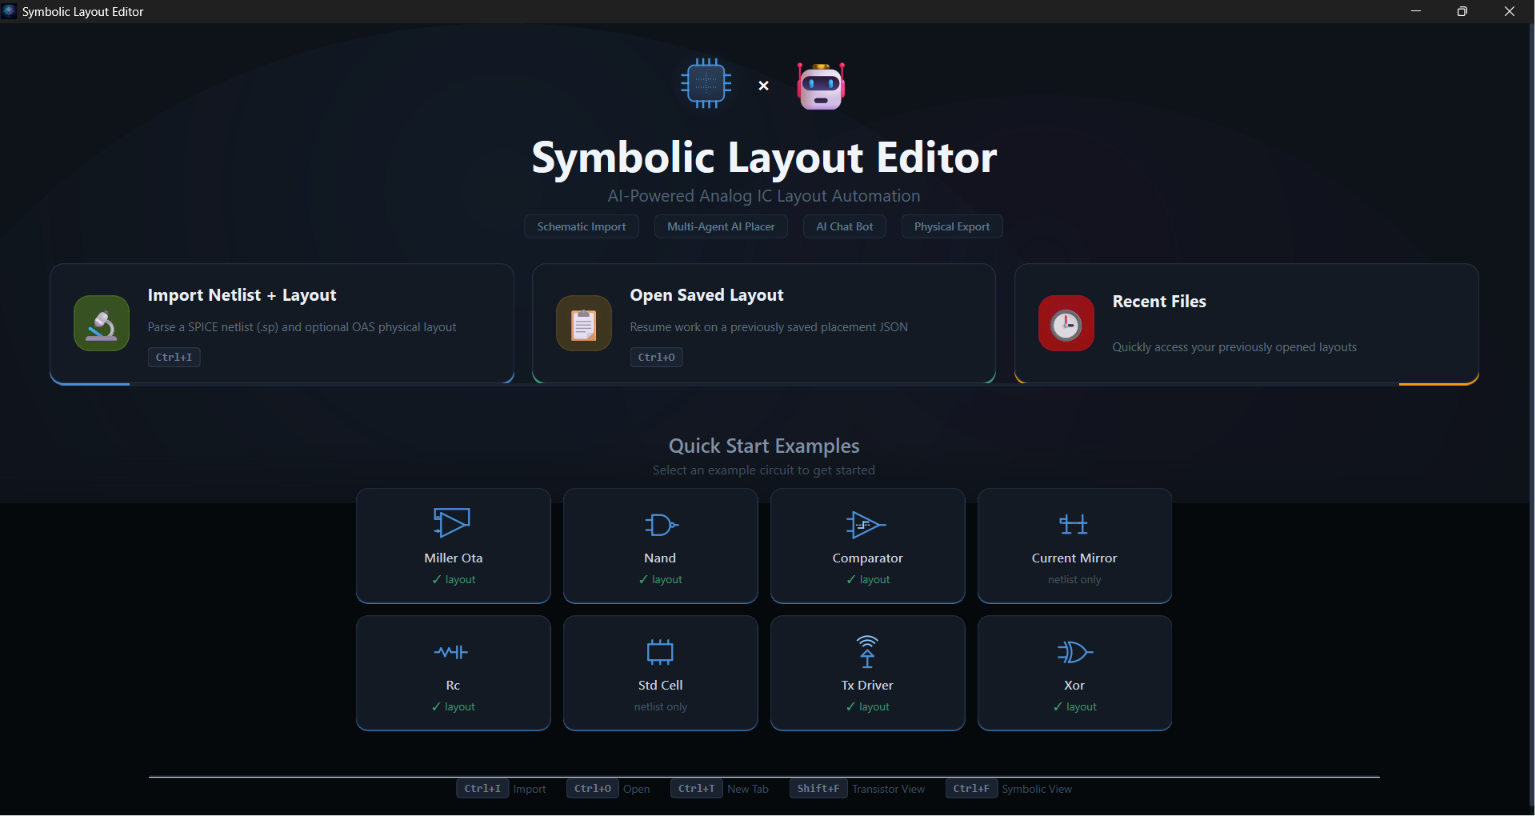
\includegraphics[width=12.5cm]{figures/GUI_Welcome_Screen.png}}
    \caption{GUI Welcome Screen dashboard of the layout automation tool, offering project initialization, SPICE netlist imports, and recent workspace reloading.}
    \label{fig:gui_welcome}
\end{figure}

\subsection{Main Interface Panels and Layout Canvas}
\noindent
The active designer workspace is organized into modular dockable panels. Figure~\ref{fig:gui_panels} illustrates the main GUI panels (\texttt{GUI\_Panals.png}) in a StrongARM dynamic comparator edit session. The workspace is divided into three primary vertical columns:
\begin{itemize}
    \item \textbf{Left Column (Design Hierarchy):} Houses the parsed device list tree, PDK parameters, and the active Schematic Assistant panel displaying the Gemini-generated schematic.
    \item \textbf{Center Column (Workspaces):} Displays the interactive symbolic placement canvas (top) and the synchronized real-time KLayout physical layout viewer (bottom).
    \item \textbf{Right Column (Co-Pilot ChatPanel):} Contains the natural language chat interface where the designer communicates layout commands and reviews critic feedback.
\end{itemize}

\noindent
The core value of this layout lies in the synchronization between the center split panels. The symbolic placement canvas (implemented as a custom interactive canvas class) allows the designer to manually drag and swap devices, set multiplier spacing, and toggle diffusion abutment. Simultaneously, a background watchdog thread detects coordinate updates, compiles them into a GDSII stream via the Gdstk backend, and redraws the physical layout in KLayout via a local TCP socket connection. This allows the designer to see how high-level symbolic changes instantly affect physical metal lines, spacing rules, and boundary guard rings.

\begin{figure}[H]
    \centering
    \fbox{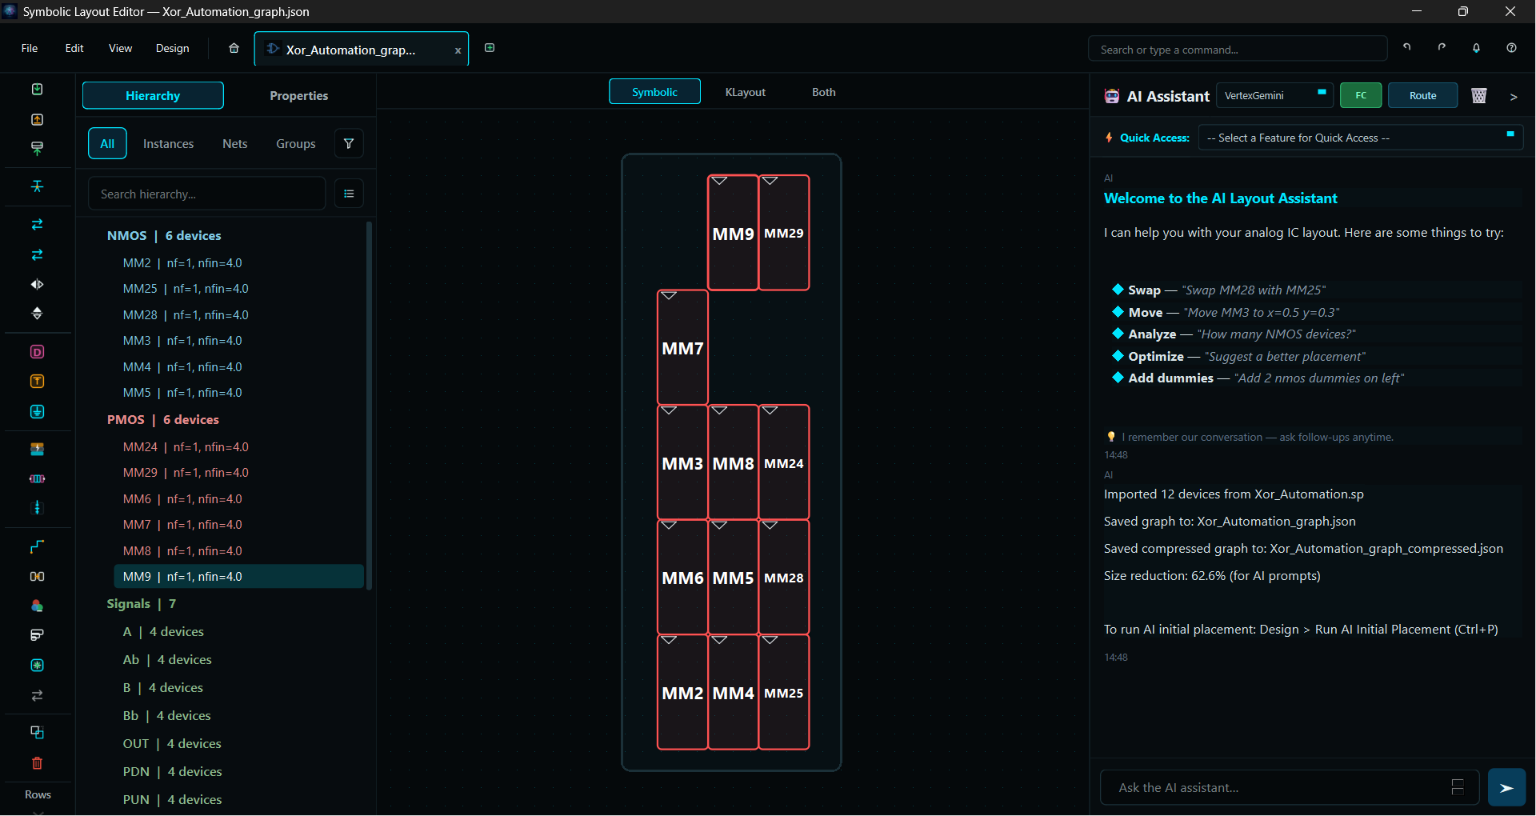
\includegraphics[width=12.5cm]{figures/GUI_Panals.png}}
    \caption{Main interface layout during an active edit session, showcasing the design tree on the left, the split symbolic and physical canvases in the center, and the ChatPanel on the right.}
    \label{fig:gui_panels}
\end{figure}

\noindent
\begin{minipage}[t]{0.60\textwidth}
    \vspace{0pt}
    \subsection{Design Panel Actions Sidebar}
    \noindent
    Figure~\ref{fig:gui_actions} shows the Design Actions Sidebar (\texttt{actions\_panal.png}) docked along the workspace. This sidebar offers quick-access buttons for core compiler pipeline commands, allowing designers to execute operations with a single click:
    \begin{itemize}
        \item \textbf{Import \& Snap:} Loads netlists and snaps transistor placements to discrete PDK coordinates.
        \item \textbf{Run Specialist Placer:} Dispatches the placement specialist agent to optimize transistor sequencing.
        \item \textbf{Enforce Symmetry:} Enforces geometric mirroring constraints across differential structures.
        \item \textbf{Verify \& Auto-Heal:} Executes sweepline check loops to detect and automatically heal spacing violations.
        \item \textbf{Export OASIS/OA:} Calls physical compaction sweeps and compiles layout streams.
    \end{itemize}
    
   
\end{minipage}
\hfill
\begin{minipage}[t]{0.15\textwidth}
    \vspace{0pt}
    \centering
    \fbox{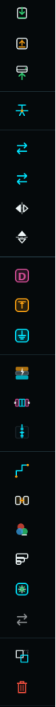
\includegraphics[height=8.5cm,keepaspectratio]{figures/actions_panal.png}}
    \captionof{figure}{GUI Design Actions Sidebar panel.}
    \label{fig:gui_actions}
\end{minipage}

\vspace{1.0cm}

\noindent
\begin{minipage}[t]{0.52\textwidth}
    \vspace{0pt}
    \subsection{Design Panel Options and Preferences}
    \noindent
    Figure~\ref{fig:gui_options} details the Design Panel Options dialog (\texttt{Design\_}\allowbreak\texttt{panal\_}\allowbreak\texttt{options.png}). It allows designers to select the target LLM provider (e.g., local Llama-3-8B vs. Vertex AI Gemini), adjust self-healing convergence thresholds, configure guard ring parameters, and toggle PDK snap grids. This preferences pane provides complete control over model execution parameters, enabling custom optimization tuning for various circuit complexities.
    
    \noindent
    By separating these settings into a persistent options dialog, the tool ensures that designers can tailor the compiler behavior to the specific PDK and target architecture. For example, when compiler synthesis is run on highly sensitive analog blocks like dynamic latches, the designer can increase the self-healing iteration limit to 5 and choose the cloud-based Vertex AI Gemini backend to ensure higher reasoning quality. For simpler digital blocks like XOR gates, switching to the locally hosted Llama-3-8B backend and reducing guard ring widths provides low-latency execution and high cell density. This level of customization ensures the framework is adaptable to both digital standard cells and precision analog blocks.
\end{minipage}
\hfill
\begin{minipage}[t]{0.42\textwidth}
    \vspace{0pt}
    \centering
    \fbox{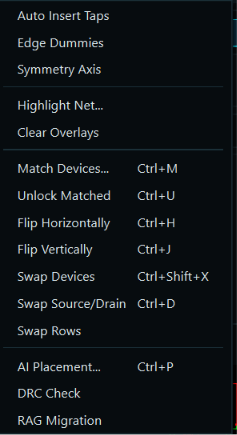
\includegraphics[width=\textwidth]{figures/Design_panal_options.png}}
    \captionof{figure}{Design panel settings dialog.}
    \label{fig:gui_options}
\end{minipage}


% ==============================================================================
\newpage	
\section[Area Reductions]{Placement Footprint \& Area Reductions}
\label{sec:area_reductions}

The layout compiler's compaction engine compresses the loose symbolic placement into a compacted physical layout. During this compaction, the compiler identifies adjacent devices sharing common electrical nets and removes the isolation clearances, allowing their active diffusions to merge.

% ------------------------------------------------------------------------------
\subsection{Benchmark Example 1: Symmetric XOR Gate Layout Synthesis}

We evaluate the synthesis process on a symmetric digital XOR Gate. This circuit block helps demonstrate standard cell layouts where parallel transistor trees are placed on a shared row height template, and signal tracks must snap to PDK coordinates.

Figure~\ref{fig:xor_before} shows the initial, unplaced representation. The transistors are arranged along default row channels on a loose grid. At this stage, no active regions are shared, and no physical compaction or routing tracks are generated.

\begin{figure}[H]
    \centering
    \fbox{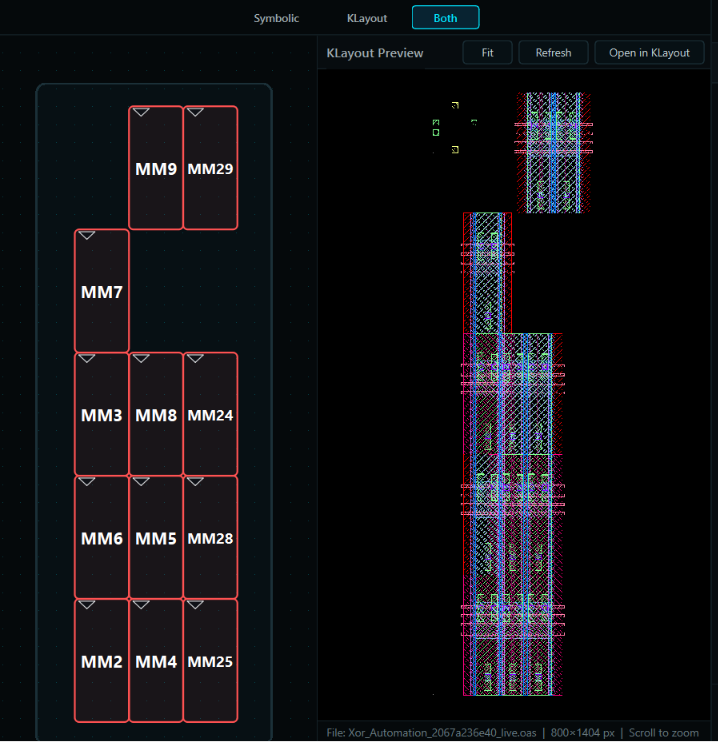
\includegraphics[width=10.5cm]{figures/xor_before_AI_placement.png}}
    \caption{Initial unplaced representation of the XOR gate in the symbolic editor, showing transistors arranged on default channels prior to compaction.}
    \label{fig:xor_before}
\end{figure}
\newpage
\noindent
In Figure~\ref{fig:xor_symbolic}, the placement agent has executed row planning and diffusion abutment. The NMOS and PMOS rows are grouped, and adjacent devices sharing common source/drain terminals are abutted (drawn adjacent to each other with active diffusions overlapping). This reduces the horizontal footprint of the layout cell.

\begin{figure}[H]
    \centering
    \fbox{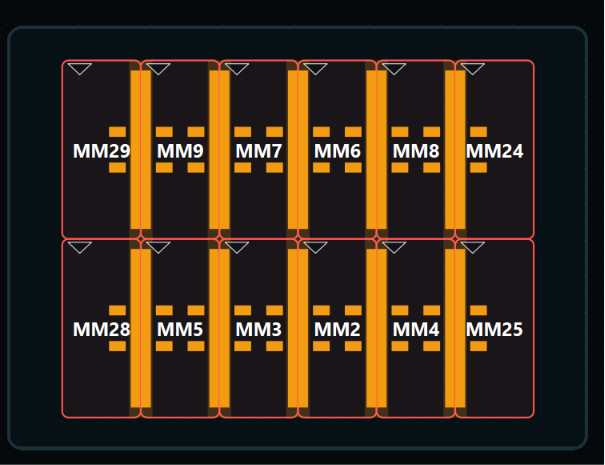
\includegraphics[width=10.5cm]{figures/xor_symbolic.png}}
    \caption{Symbolic placement of the XOR gate showing active region sharing.}
    \label{fig:xor_symbolic}
\end{figure}

Figure~\ref{fig:xor_schematic} displays the transistor-level schematic of the XOR gate. 

\begin{figure}[H]
    \centering
    \fbox{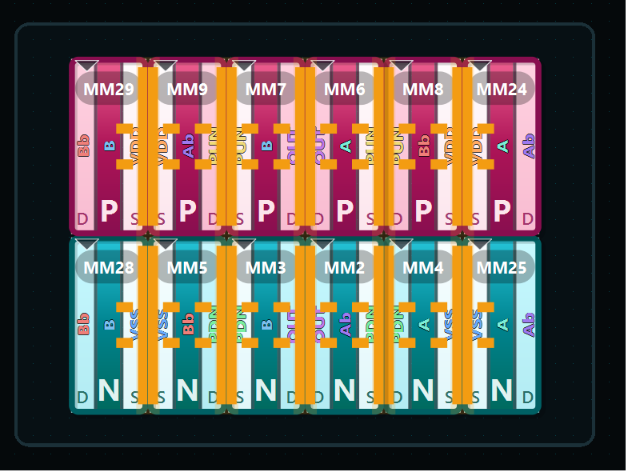
\includegraphics[width=10.5cm]{figures/xor_transistor_level.png}}
    \caption{Transistor-level schematic of the benchmark XOR gate.}
    \label{fig:xor_schematic}
\end{figure}
\newpage
\noindent
Figure~\ref{fig:xor_sch_ai} shows the corresponding AI-generated schematic layout produced by the Schematic Assistant. The assistant automatically groups PMOS devices at the top ($y < 0$) and NMOS devices at the bottom ($y \geq 0$) to align with current flow, routing local interconnects as solid Manhattan wires.

\noindent
The generated schematic illustrates a clean vertical partition between the PMOS pull-up network and the NMOS pull-down network, mirroring standard IC design textbook conventions. Internal nodes (such as the gate inputs and local source-drain bridges) are rendered as short, direct Manhattan wire segments, while primary inputs and power connections are labeled at the cell borders.  connectivity matches the SPICE netlist structure, prior to committing the layout to physical compilation.

\begin{figure}[H]
    \centering
    \fbox{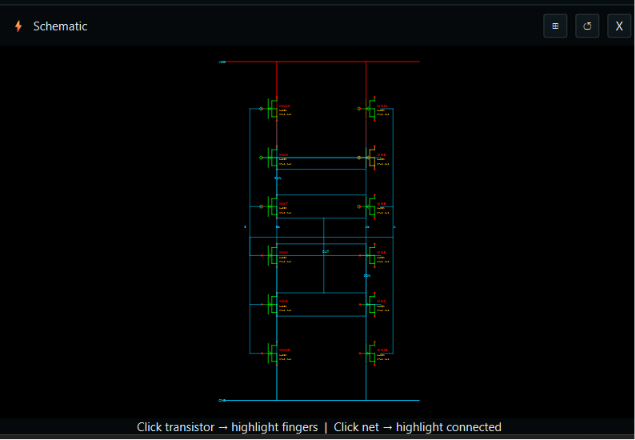
\includegraphics[width=12.5cm]{figures/xor_sch_AI_generated.png}}
    \caption{AI-generated schematic layout of the XOR gate in the Schematic Assistant, showing top-to-bottom PMOS-NMOS vertical stacking and local node routing.}
    \label{fig:xor_sch_ai}
\end{figure}
\newpage
\noindent
The final physical layout compiled to GDSII and rendered in KLayout is shown in Figure~\ref{fig:xor_klayout}. Devices are placed at their final physical coordinates, with active source/drain regions merged, and routing wires snapped to Metal 1 and Metal 2 tracks.

\begin{figure}[H]
    \centering
    \fbox{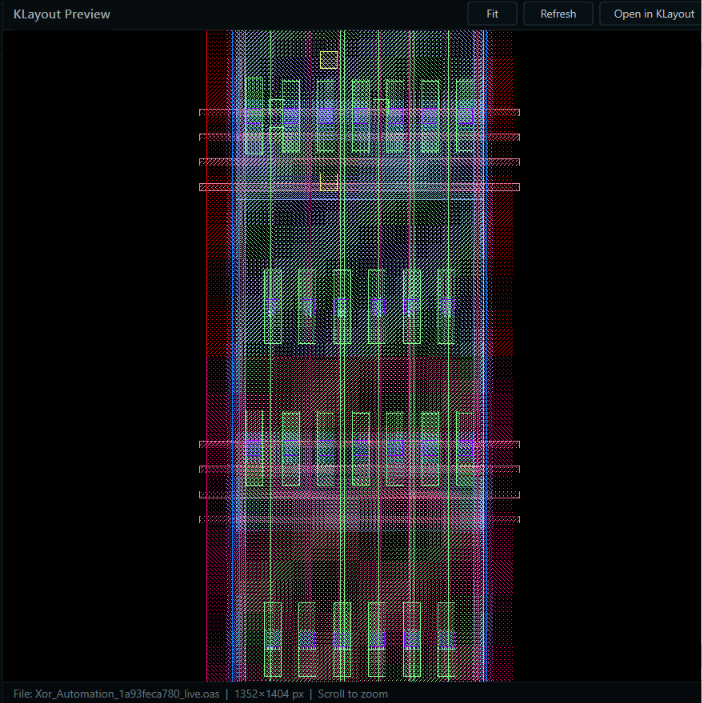
\includegraphics[width=11.5cm]{figures/xor_klayout.png}}
    \caption{Final compacted and routed physical layout of the XOR gate cell in KLayout, showing snapped Metal 1/2 routing tracks and boundary clearances.}
    \label{fig:xor_klayout}
\end{figure}

\clearpage

% ------------------------------------------------------------------------------
\subsection{Benchmark Example 2: 2-Transistor Current Mirror Layout Synthesis}

The 2-Transistor Current Mirror is a fundamental analog matching cell. It requires symmetrical layout matching, dummy transistor insertion on the boundaries, and active diffusion sharing to reduce mismatch.

Figure~\ref{fig:cm_before} shows the current mirror in the unplaced stage. The devices are positioned on the symbolic grid with default clearances, leaving their active diffusions completely isolated.

\begin{figure}[H]
    \centering
    \fbox{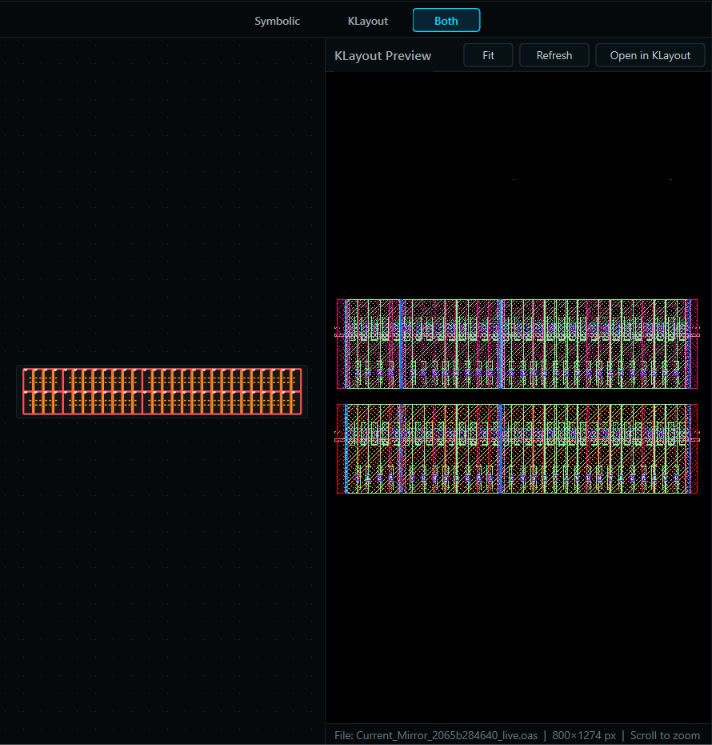
\includegraphics[width=10.5cm]{figures/current_mirror_before_AI_placement.png}}
    \caption{Initial uncompacted placement of the 2-Transistor Current Mirror block, showing wide device separation and isolated active areas.}
    \label{fig:cm_before}
\end{figure}

\newpage
\noindent
Figure~\ref{fig:cm_symbolic} shows the symbolic placement with active abutment enabled. The NMOS source terminals are joined, enabling the compiler to merge their active diffusions and remove the default isolation spaces.

\begin{figure}[H]
    \centering
    \fbox{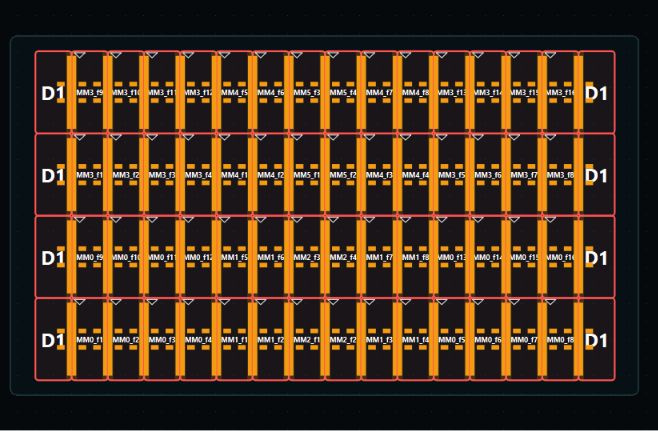
\includegraphics[width=11.5cm]{figures/current_mirror_symbolic.png}}
    \caption{Symbolic placement of the Current Mirror with active diffusion sharing (abutment) and boundary guard ring outlines.}
    \label{fig:cm_symbolic}
\end{figure}
\noindent
Figure~\ref{fig:cm_schematic} displays the transistor-level schematic of the current mirror, highlighting the matched gate connections and the common source ground node.

\begin{figure}[H]
    \centering
    \fbox{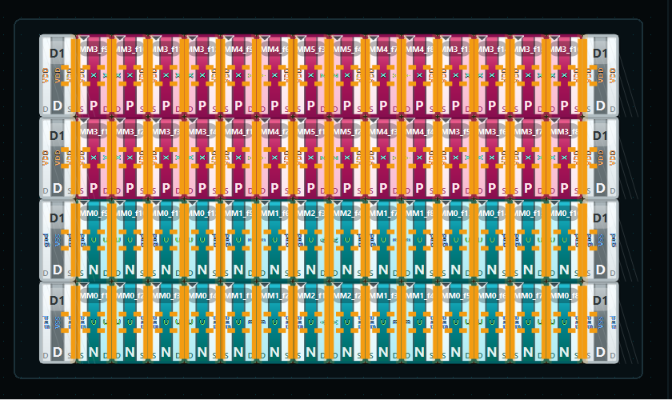
\includegraphics[width=11.5cm]{figures/current_mirror_transistor_level.png}}
    \caption{Transistor-level schematic of the current mirror block showing gate matching and shared ground connections.}
    \label{fig:cm_schematic}
\end{figure}
\newpage
\noindent
Figure~\ref{fig:cm_schematic_colored} shows the color-coded schematic highlighting the common-centroid-like matching patterns. Devices are grouped and color-coded to visualize the routing tracks and dummy transistor assignments.

\begin{figure}[H]
    \centering
    \fbox{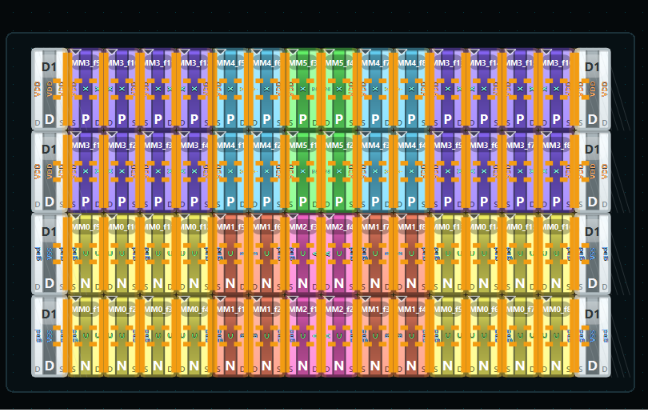
\includegraphics[width=10.5cm]{figures/current_mirror_transistor_level_colord.png}}
    \caption{Color-coded transistor-level schematic detailing the matching patterns and common centroid routing plans for the current mirror.}
    \label{fig:cm_schematic_colored}
\end{figure}
\noindent
Figure~\ref{fig:cm_klayout} illustrates the final compacted GDSII cell layout in KLayout. 

\begin{figure}[H]
    \centering
    \fbox{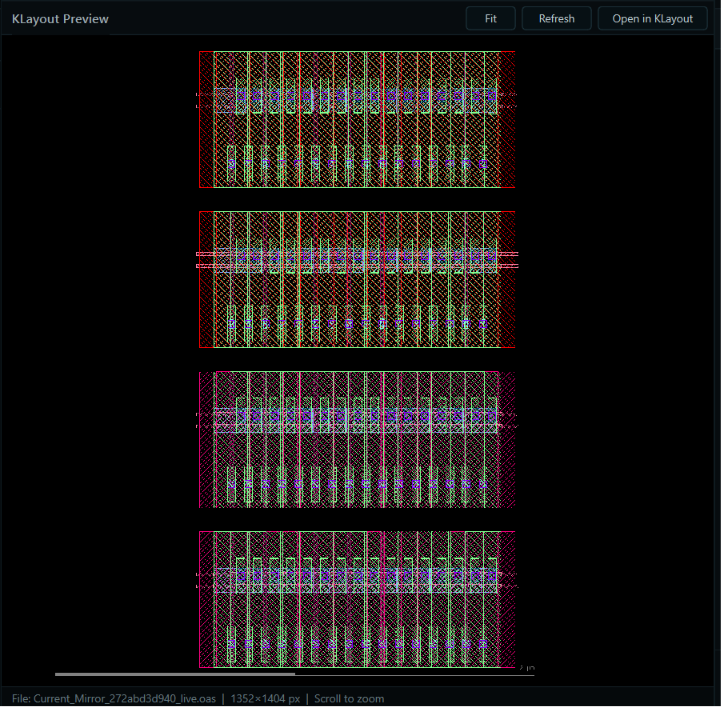
\includegraphics[width=10.5cm]{figures/current_mirror_klayout.png}}
    \caption{Final compacted GDSII cell layout of the current mirror in KLayout, showing shared diffusion regions and gate poly tracks.}
    \label{fig:cm_klayout}
\end{figure}
\newpage
\noindent
Figure~\ref{fig:cm_cc} displays the cell imported into Synopsys Custom Compiler via the OpenAccess TCL exporter. The watchdog script matches design parameters, moves devices, and synchronizes connectivity.

\begin{figure}[H]
    \centering
    \fbox{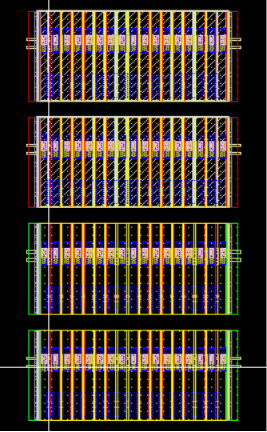
\includegraphics[width=10.5cm]{figures/current_mirror_from_custom_compiler.png}}
    \caption{Native cellview of the Current Mirror successfully imported into Synopsys Custom Compiler via watchdog-triggered OpenAccess script injection.}
    \label{fig:cm_cc}
\end{figure}

\clearpage

% ------------------------------------------------------------------------------
\subsection{Benchmark Example 3: Dynamic Analog Comparator Layout Synthesis}

The Dynamic Analog Comparator is a complex mixed-signal cell combining an input differential pair, a cross-coupled regenerative latch, and clock gating transistors. It has a high density of interconnects and strict symmetry requirements.

Figure~\ref{fig:comp_before} shows the unplaced comparator devices. The devices are positioned on the symbolic grid with wide clearances to avoid design rule violations.

\begin{figure}[H]
    \centering
    \fbox{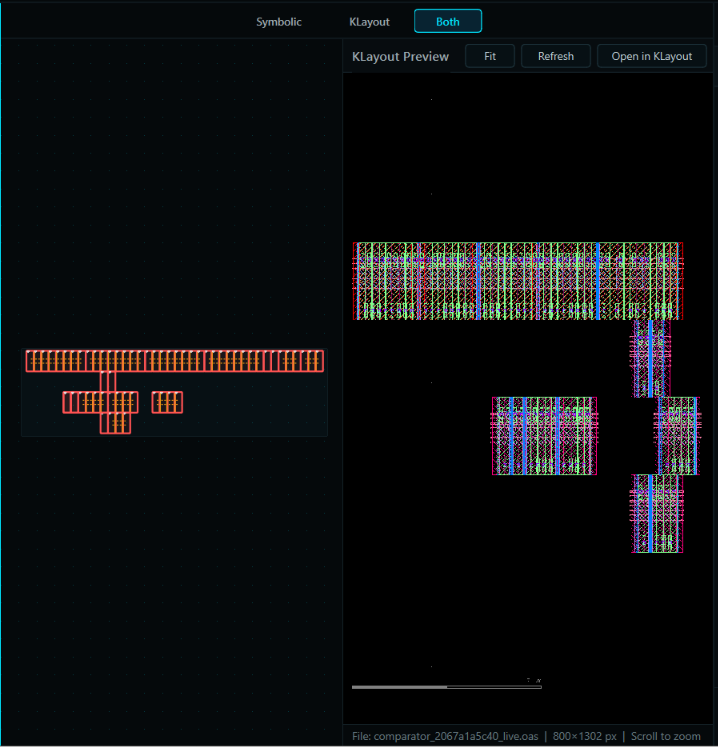
\includegraphics[width=10.5cm]{figures/comparator_before_AI_placement.png}}
    \caption{Initial uncompacted symbolic placement of the Dynamic Analog Comparator cell, showing the latch and input pair layout template.}
    \label{fig:comp_before}
\end{figure}
\noindent
Figure~\ref{fig:comparator_sch_ai} shows the corresponding AI-generated schematic layout produced by the Schematic Assistant. The assistant coordinates the placement of the StrongARM latch branches, mapping the precharge PMOS, NMOS/PMOS latch pairs, input differential pair, and tail gating transistor to clear vertical ranks ($y = -2, -1, 0, 1, 2$) and generating the cross-coupled X-shaped feedback lines.

\noindent
Due to the high interconnect density and regenerative feedback loops characteristic of StrongARM comparators, automatic schematic drafting is notoriously difficult for standard graph-drawing heuristics. The Schematic Assistant resolves this by enforcing structural constraints in the prompt: matching NMOS and PMOS latch pairs face each other, input pairs are mirrored across the $x=0$ axis, and tail bias devices are centered at the bottom. The resulting canvas displays two distinct, symmetric branches with the cross-coupled gates linked by a clear, overlapping ``X'' wire configuration. Selecting any component in this schematic immediately highlights the respective fingers and routing wires in the physical viewer, showing how the physical symmetries match the schematic planning.

\begin{figure}[H]
    \centering
    \fbox{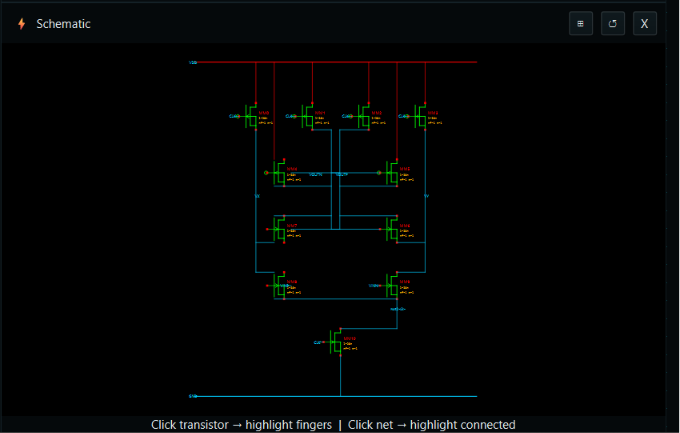
\includegraphics[width=10.5cm]{figures/comparator_sch_AI_generated.png}}
    \caption{AI-generated schematic layout of the Dynamic Analog Comparator in the Schematic Assistant, showcasing differential input pair matching, cross-coupled latch cross-wiring, and precharge gating.}
    \label{fig:comparator_sch_ai}
\end{figure}



\begin{figure}[H]
    \centering
    \fbox{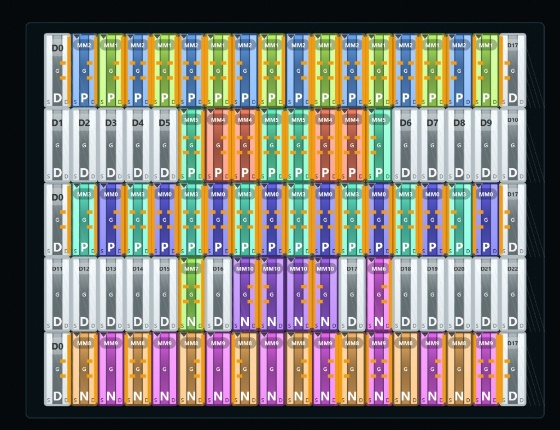
\includegraphics[width=10.5cm]{figures/Comparator.png}}
    \caption{Final compacted physical layout of the Dynamic Analog Comparator cell, showing symmetrical device placement.}
    \label{fig:comp_klayout}
\end{figure}

\clearpage% ------------------------------------------------------------------------------



